%%%%%%%%%%%%%%%%%%%%%%%%%%%%%%%%%%%%%%%%%%%%%%%%%%%%%%%%%%%%%%%%%%%%%%%%%%%%%%%%
%%% Author: https://github.com/jtleek/capitalIn21stCenturyinR
%%% Author: knitr/beamer by Patrick Toche, December 2014
%%% Author: data/content by Thomas Piketty, 2013-2014
%%% This replicates a December 2014 presentation at Sao Paulo by Thomas Piketty
%%% The .Rnw file is the 'master', other files produced by knitr compilation
%%% To compile in R: library(knitr); knit("slides.Rnw");
%%% To compile in Rstudio: 'Compile PDF' menu command
%%% The 'pictures' directory contains images inserted with \includegraphics
%%% The 'figures' directory contains pdf created and inserted by knitr
%%% Delete the 'cache' directory to recreate pdf graphics
%%% The 'SaoPaulo' directory contains pdf of original powerpoint for reference
%%%%%%%%%%%%%%%%%%%%%%%%%%%%%%%%%%%%%%%%%%%%%%%%%%%%%%%%%%%%%%%%%%%%%%%%%%%%%%%%

%%% \PassOptionsToPackage loads options for packages loaded by beamer class
\PassOptionsToPackage{obeyspaces}{url}% url package loaded by hyperref
\PassOptionsToPackage{usenames,dvipsnames,svgnames}{xcolor}% named colors
\PassOptionsToPackage{%
    unicode = {false}%
    , colorlinks = {true}%
    , linkcolor = {MidnightBlue}%
    , filecolor = {MidnightBlue}%
    , citecolor = {MidnightBlue}%
    , urlcolor = {MidnightBlue}%
    , breaklinks = {false}%
    , plainpages = {true}% page number anchors as plain arabic
    , bookmarks = {true}%
    , bookmarksnumbered = {true}%
    , bookmarksopen = {true}%
    , backref = {false}%
    , pdfusetitle = {true}%
    , pdfpagemode = {UseNone}% UseThumbs, UseOutlines, FullScreen, UseNone
    , pdfpagetransition = {Wipe /Di -45}%
    , pdfpagelayout = {SinglePage}%
    , pdfpagelabels = {false}% fix for beamer bug for some classes
    , pdfstartpage = {1}%
    , pdfstartview = {FitV}%
    , pdffitwindow = {false}%
    , pdfcenterwindow = {true}%
    , pdfmenubar = {true}%
    , pdfdisplaydoctitle = {true}%
}{hyperref}

%%%%%%%%%% Preamble Here %%%%%%%%%%%%%%%%%%%%%%%%%%%%%%%%%%%%%%%%%%%%%%%%%%%%%%%
\documentclass[t]{beamer}\usepackage[]{graphicx}\usepackage[]{color}
%% maxwidth is the original width if it is less than linewidth
%% otherwise use linewidth (to make sure the graphics do not exceed the margin)
\makeatletter
\def\maxwidth{ %
  \ifdim\Gin@nat@width>\linewidth
    \linewidth
  \else
    \Gin@nat@width
  \fi
}
\makeatother

\definecolor{fgcolor}{rgb}{0.345, 0.345, 0.345}
\newcommand{\hlnum}[1]{\textcolor[rgb]{0.686,0.059,0.569}{#1}}%
\newcommand{\hlstr}[1]{\textcolor[rgb]{0.192,0.494,0.8}{#1}}%
\newcommand{\hlcom}[1]{\textcolor[rgb]{0.678,0.584,0.686}{\textit{#1}}}%
\newcommand{\hlopt}[1]{\textcolor[rgb]{0,0,0}{#1}}%
\newcommand{\hlstd}[1]{\textcolor[rgb]{0.345,0.345,0.345}{#1}}%
\newcommand{\hlkwa}[1]{\textcolor[rgb]{0.161,0.373,0.58}{\textbf{#1}}}%
\newcommand{\hlkwb}[1]{\textcolor[rgb]{0.69,0.353,0.396}{#1}}%
\newcommand{\hlkwc}[1]{\textcolor[rgb]{0.333,0.667,0.333}{#1}}%
\newcommand{\hlkwd}[1]{\textcolor[rgb]{0.737,0.353,0.396}{\textbf{#1}}}%

\usepackage{framed}
\makeatletter
\newenvironment{kframe}{%
 \def\at@end@of@kframe{}%
 \ifinner\ifhmode%
  \def\at@end@of@kframe{\end{minipage}}%
  \begin{minipage}{\columnwidth}%
 \fi\fi%
 \def\FrameCommand##1{\hskip\@totalleftmargin \hskip-\fboxsep
 \colorbox{shadecolor}{##1}\hskip-\fboxsep
     % There is no \\@totalrightmargin, so:
     \hskip-\linewidth \hskip-\@totalleftmargin \hskip\columnwidth}%
 \MakeFramed {\advance\hsize-\width
   \@totalleftmargin\z@ \linewidth\hsize
   \@setminipage}}%
 {\par\unskip\endMakeFramed%
 \at@end@of@kframe}
\makeatother

\definecolor{shadecolor}{rgb}{.97, .97, .97}
\definecolor{messagecolor}{rgb}{0, 0, 0}
\definecolor{warningcolor}{rgb}{1, 0, 1}
\definecolor{errorcolor}{rgb}{1, 0, 0}
\newenvironment{knitrout}{}{} % an empty environment to be redefined in TeX

\usepackage{alltt}

%%%%%%%%%% Set Document Information %%%%%%%%%%%%%%%%%%%%%%%%%%%%%%%%%%%%%%%%%%%%
\title{Capital in the 21st Century}
\author[Thomas Piketty]{Thomas Piketty\inst{1}\inst{2}}
\institute{$^1$Paris School of Economics \\
  Sao Paulo, 26 November 2014 \bigskip\bigskip \\
  $^2$translated to beamer via knitr by Patrick Toche \\
  \href{mailto:contact@patricktoche.com}{contact@patricktoche.com} \\
  Based on collaborative effort led by Jeff Leek \\
  \url{https://github.com/jtleek/capitalIn21stCenturyinR} \\
  All copyright claims with Professor Piketty
}
\date{December 2014}

%%%%%%%%%% Set Beamer Options %%%%%%%%%%%%%%%%%%%%%%%%%%%%%%%%%%%%%%%%%%%%%%%%%%
\usetheme{piketty}

%%%%%%%%%% Load Latex Packages %%%%%%%%%%%%%%%%%%%%%%%%%%%%%%%%%%%%%%%%%%%%%%%%%
\usepackage[T1]{fontenc}
\usepackage{lmodern}
\usepackage{booktabs}
\usepackage[flushleft]{threeparttable}
\usepackage{adjustbox}

%%%%%%%%%% Set Miscellani %%%%%%%%%%%%%%%%%%%%%%%%%%%%%%%%%%%%%%%%%%%%%%%%%%%%%%
\setcounter{secnumdepth}{3}%
\setcounter{tocdepth}{3}%
\setlength{\abovecaptionskip}{0pt}%
\setlength{\belowcaptionskip}{0pt}%

%%%%%%%%%% Load knitr Options %%%%%%%%%%%%%%%%%%%%%%%%%%%%%%%%%%%%%%%%%%%%%%%%%%



%%%%%%%%%% Start of Document %%%%%%%%%%%%%%%%%%%%%%%%%%%%%%%%%%%%%%%%%%%%%%%%%%%
\IfFileExists{upquote.sty}{\usepackage{upquote}}{}
\begin{document}

% first slide with title/author information
\maketitle

%%%%%%%%%%%%%%%%%%%% Frame Here %%%%%%%%%%%%%%%%%%%%%%%%%%%%%%%%%%%%%%%%%%%%%%%%
\begin{frame}[label=Introduction1]
\begin{itemize}
\item
This presentation is based upon Capital in the 21st century (Harvard University Press, March 2014)
\item
This book studies the global dynamics of income and wealth distribution since 18c in 20+ countries; I use historical data collected over the past 15 years with Atkinson, Saez, Postel-Vinay, Rosenthal, Alvaredo, Zucman, and 30+ others; I try to shift attention from rising income inequality to rising wealth inequality
\item
The book includes four parts:
\begin{itemize}
\item
Part 1. Income and capital
\item
Part 2. The dynamics of the capital/income ratio 
\item
Part 3. The structure of inequalities
\item
Part 4. Regulating capital in the 21st century
\end{itemize}
\item 
In this presentation I will present some results from Parts 2 \& 3, focusing upon the long-run evolution of capital/income ratios and wealth concentration (all graphs and series are available on line:
see http://piketty.pse.ens.fr/capital21c)
\end{itemize}
\end{frame}
%%%%%%%%%%%%%%%%%%%% Frame Here %%%%%%%%%%%%%%%%%%%%%%%%%%%%%%%%%%%%%%%%%%%%%%%%


%%%%%%%%%%%%%%%%%%%% Frame Here %%%%%%%%%%%%%%%%%%%%%%%%%%%%%%%%%%%%%%%%%%%%%%%%
\begin{frame}[label=WTID]
\frametitle{The World Top Incomes Database}
\begin{figure}[t]
\begin{minipage}[b]{\textwidth}
\centering
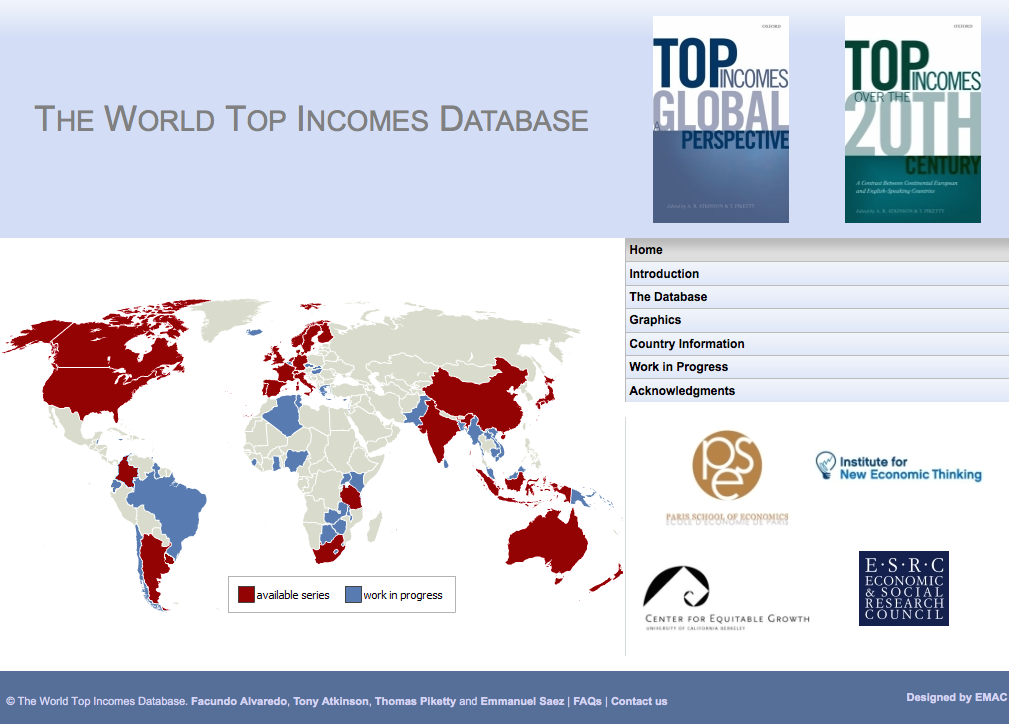
\includegraphics[width=0.9\textwidth]
{pictures/WorldTopIncomesDatabase}
\caption{\textbf{\url{http://topincomes.parisschoolofeconomics.eu}}}
\end{minipage}
\end{figure}
\end{frame}
%%%%%%%%%%%%%%%%%%%% Frame Here %%%%%%%%%%%%%%%%%%%%%%%%%%%%%%%%%%%%%%%%%%%%%%%%


%%%%%%%%%%%%%%%%%%%% Frame Here %%%%%%%%%%%%%%%%%%%%%%%%%%%%%%%%%%%%%%%%%%%%%%%%
\begin{frame}[label=Fig11,fragile]
\frametitle{Figure 1.1. Income inequality in the United States, 1910-2012}
\begin{figure}[t]
\begin{minipage}[b]{\textwidth}
\centering
\begin{knitrout}\footnotesize
\definecolor{shadecolor}{rgb}{0.969, 0.969, 0.969}\color{fgcolor}

{\centering 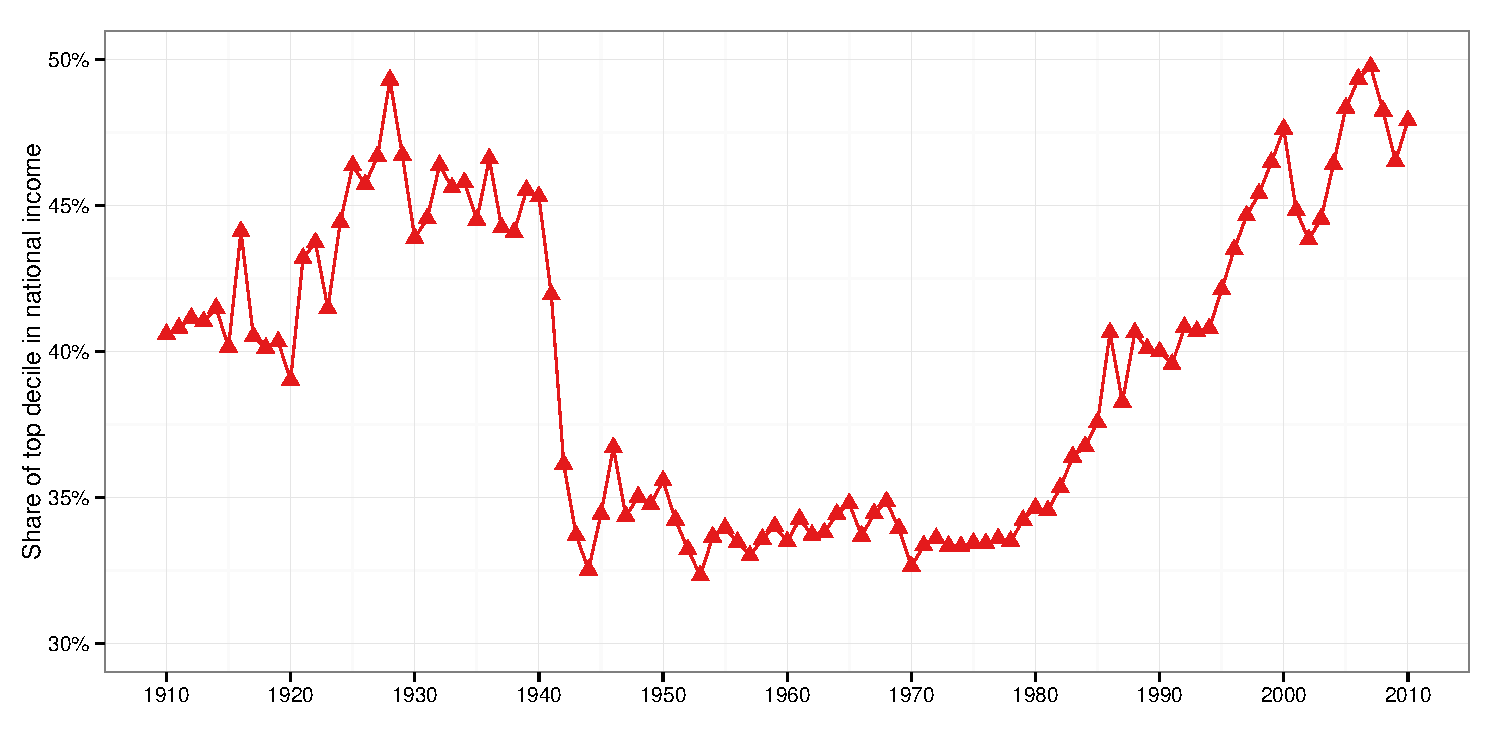
\includegraphics[width=1\linewidth]{figures/color/Figure_1_1} 

}



\end{knitrout}
\caption{The top decile share in U.S. national income dropped from 45--50\% in the 1910s--1920s to less than 35\% in the 1950s (this is the
1950 1960 fall documented by Kuznets); it then rose from less than 35\% in the 1970s to 45--50\% in the 2000s--2010s.}
\end{minipage}
\end{figure}
\end{frame}
%%%%%%%%%%%%%%%%%%%% Frame Here %%%%%%%%%%%%%%%%%%%%%%%%%%%%%%%%%%%%%%%%%%%%%%%%



%%%%%%%%%%%%%%%%%%%% Frame Here %%%%%%%%%%%%%%%%%%%%%%%%%%%%%%%%%%%%%%%%%%%%%%%%
\begin{frame}[label=Fig85,fragile]
\frametitle{Figure 1.1/8.5. Income inequality in the United States, 1910-2012}
\begin{figure}[t]
\begin{minipage}[b]{\textwidth}
\centering
\begin{knitrout}\footnotesize
\definecolor{shadecolor}{rgb}{0.969, 0.969, 0.969}\color{fgcolor}

{\centering 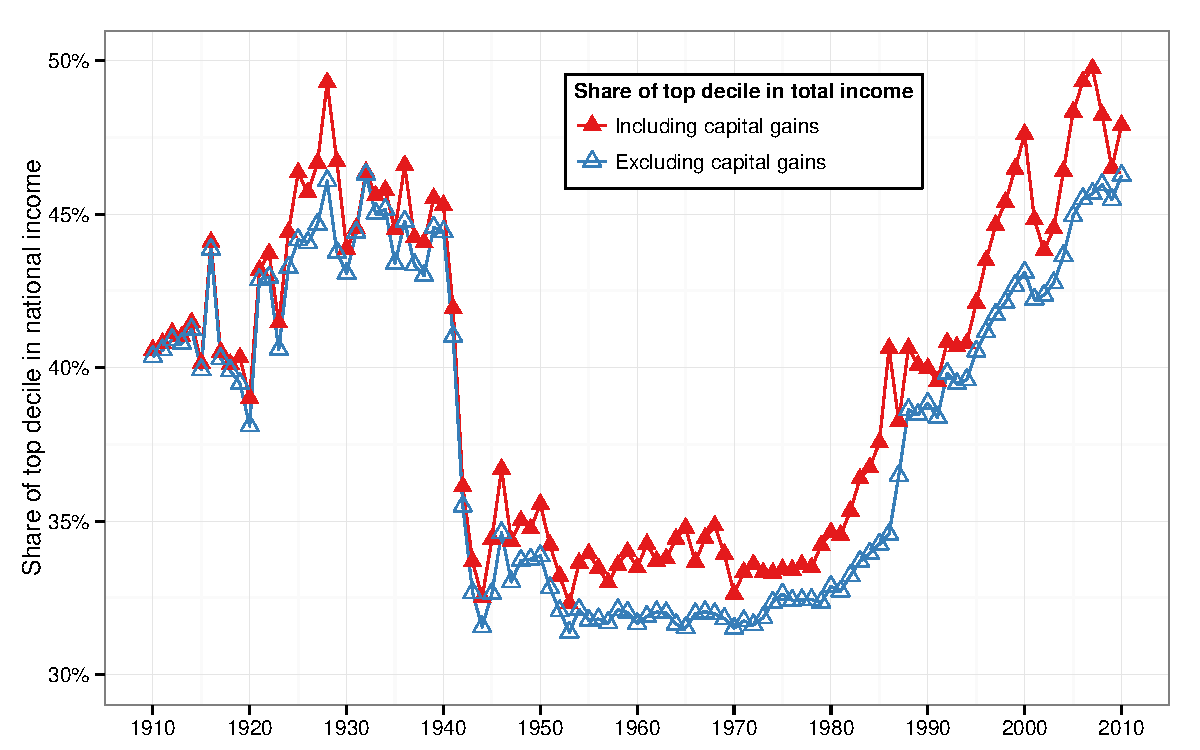
\includegraphics[width=1\linewidth]{figures/color/Figure_8_5} 

}



\end{knitrout}
\caption{The top decile share in U.S. national income dropped from 45--50\% in the 1910s--1920s to less than 35\% in the 1950s (this is the
1950 1960 fall documented by Kuznets); it then rose from less than 35\% in the 1970s to 45--50\% in the 2000s--2010s. This is actually Figure 8.5 in the book.}
\end{minipage}
\end{figure}
\end{frame}
%%%%%%%%%%%%%%%%%%%% Frame Here %%%%%%%%%%%%%%%%%%%%%%%%%%%%%%%%%%%%%%%%%%%%%%%%


%%%%%%%%%%%%%%%%%%%% Frame Here %%%%%%%%%%%%%%%%%%%%%%%%%%%%%%%%%%%%%%%%%%%%%%%%
\begin{frame}[label=Fig12,fragile]
\frametitle{Figure 1.2. The capital-income ratio in Europe, 1870-2012}
\begin{figure}[t]
\begin{minipage}[b]{\textwidth}
\centering
\begin{knitrout}\footnotesize
\definecolor{shadecolor}{rgb}{0.969, 0.969, 0.969}\color{fgcolor}

{\centering 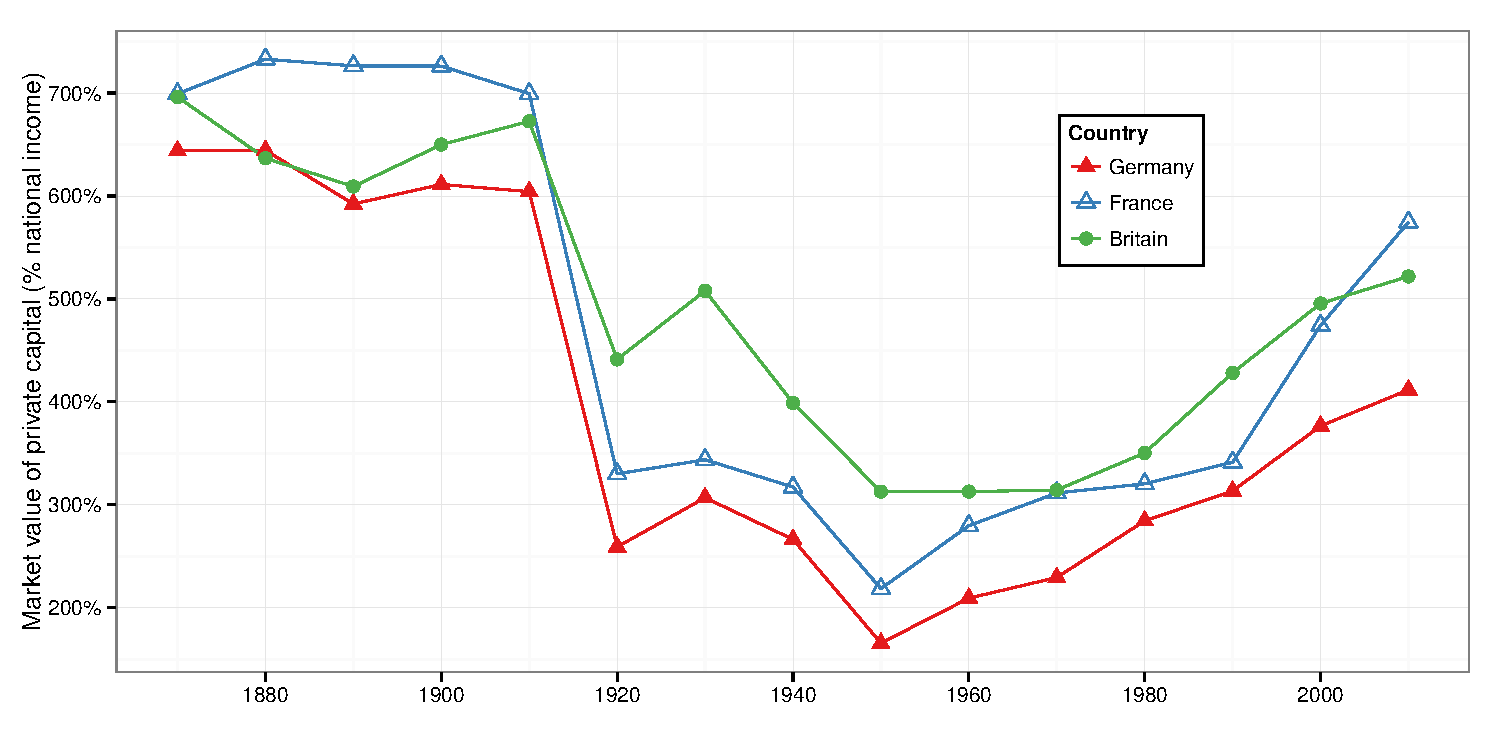
\includegraphics[width=1\linewidth]{figures/color/Figure_1_2} 

}



\end{knitrout}
\caption{Aggregate private wealth was worth about 6--7 years of national income in Europe in 1910, between 2 and 3 years in 1950, and between 4 and 6 years in 2010.}
\end{minipage}
\end{figure}
\end{frame}
%%%%%%%%%%%%%%%%%%%% Frame Here %%%%%%%%%%%%%%%%%%%%%%%%%%%%%%%%%%%%%%%%%%%%%%%%


%%%%%%%%%%%%%%%%%%%% Frame Here %%%%%%%%%%%%%%%%%%%%%%%%%%%%%%%%%%%%%%%%%%%%%%%%
\begin{frame}[label=ThreePoints,fragile]
\frametitle{This presentation: three points}
\begin{enumerate}
\item
The return of a patrimonial (or wealth-based) society in the Old World (Europe, Japan). Wealth-income ratios seem to be returning to very high levels in low growth countries.
\medskip\newline
Intuition: in a slow-growth society, wealth accumulated in the past can naturally become very important. In the very long run, this can be relevant for the entire world.
\item 
The future of wealth concentration: with high r-g during 21c (r = `net-of-tax rate of return', g = `growth rate'), then wealth inequality might reach or surpass 19c oligarchic levels; conversely, suitable institutions can allow to democratize wealth.
\item
Inequality in America (``meritocratic extremism''): is the New World developing a new inequality model that is based upon extreme labor income inequality more than upon wealth inequality? Is it more merit-based, or can it become the worst of all worlds?
\end{enumerate}
\end{frame}
%%%%%%%%%%%%%%%%%%%% Frame Here %%%%%%%%%%%%%%%%%%%%%%%%%%%%%%%%%%%%%%%%%%%%%%%%


%%%%%%%%%%%%%%%%%%%% Frame Here %%%%%%%%%%%%%%%%%%%%%%%%%%%%%%%%%%%%%%%%%%%%%%%%
\begin{frame}[label=BrasilVersus]
\frametitle{Brasil vs Europe--US--Japan}
\begin{itemize}
\item
Top income shares: income inequality is known to be high in Brasil; but it is probably underestimated (problem with household surveys); little access to fiscal data in Brasil
\item 
Wealth-income ratios: probably a strong rise in Brasil (real estate prices), but we do not really know
\item
Wealth inequality: probably very high, but we do not really know; no access to property tax and inheritance tax statistics
\item
Like other countries, Brasil needs more transparency about income and wealth; progressive tax on income, inheritance and wealth would be a powerful way to produce information about how the different income and wealth groups are benefiting from growth
\end{itemize}
\end{frame}
%%%%%%%%%%%%%%%%%%%% Frame Here %%%%%%%%%%%%%%%%%%%%%%%%%%%%%%%%%%%%%%%%%%%%%%%%


%%%%%%%%%%%%%%%%%%%% Frame Here %%%%%%%%%%%%%%%%%%%%%%%%%%%%%%%%%%%%%%%%%%%%%%%%
\begin{frame}[label=BrazilUSTop1]
\frametitle{Top 1\% income share: Brazil and US, 2006--2012}
\begin{figure}[t]
\begin{minipage}[b]{\textwidth}
\centering
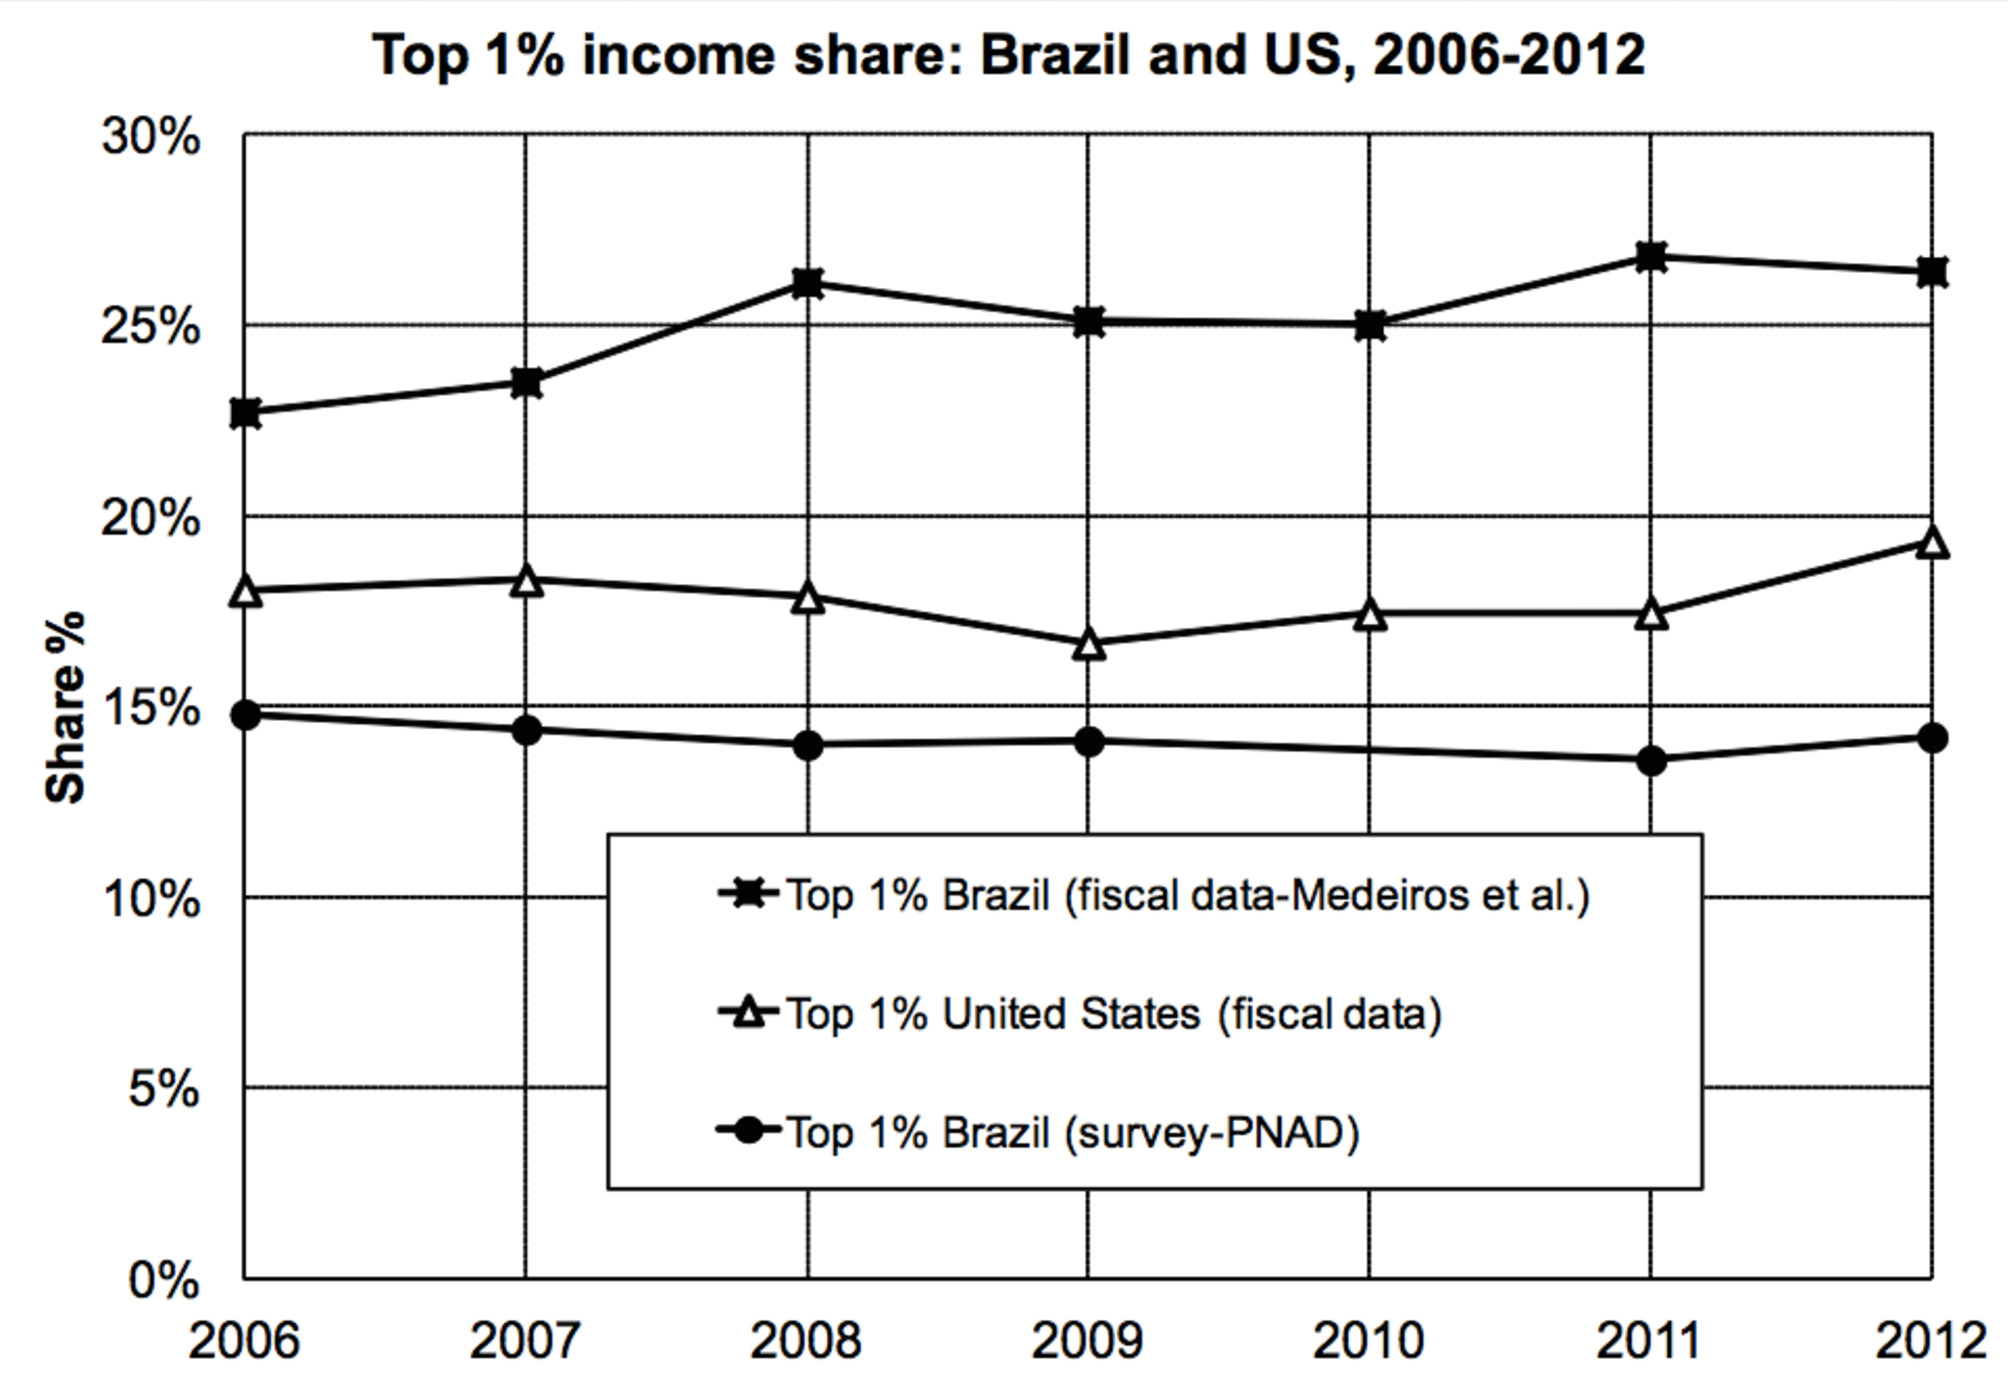
\includegraphics[width=\textwidth]
{pictures/Top1BrazilVsUSA}
\caption{To Do: Get Data to Recreate Figure}
\end{minipage}
\end{figure}
\end{frame}
%%%%%%%%%%%%%%%%%%%% Frame Here %%%%%%%%%%%%%%%%%%%%%%%%%%%%%%%%%%%%%%%%%%%%%%%%


%%%%%%%%%%%%%%%%%%%% Frame Here %%%%%%%%%%%%%%%%%%%%%%%%%%%%%%%%%%%%%%%%%%%%%%%%
\begin{frame}[label=BrazilUSTop10]
\frametitle{Top 10\% income share: Brazil and US, 2006--2012}
\begin{figure}[t]
\begin{minipage}[b]{\textwidth}
\centering
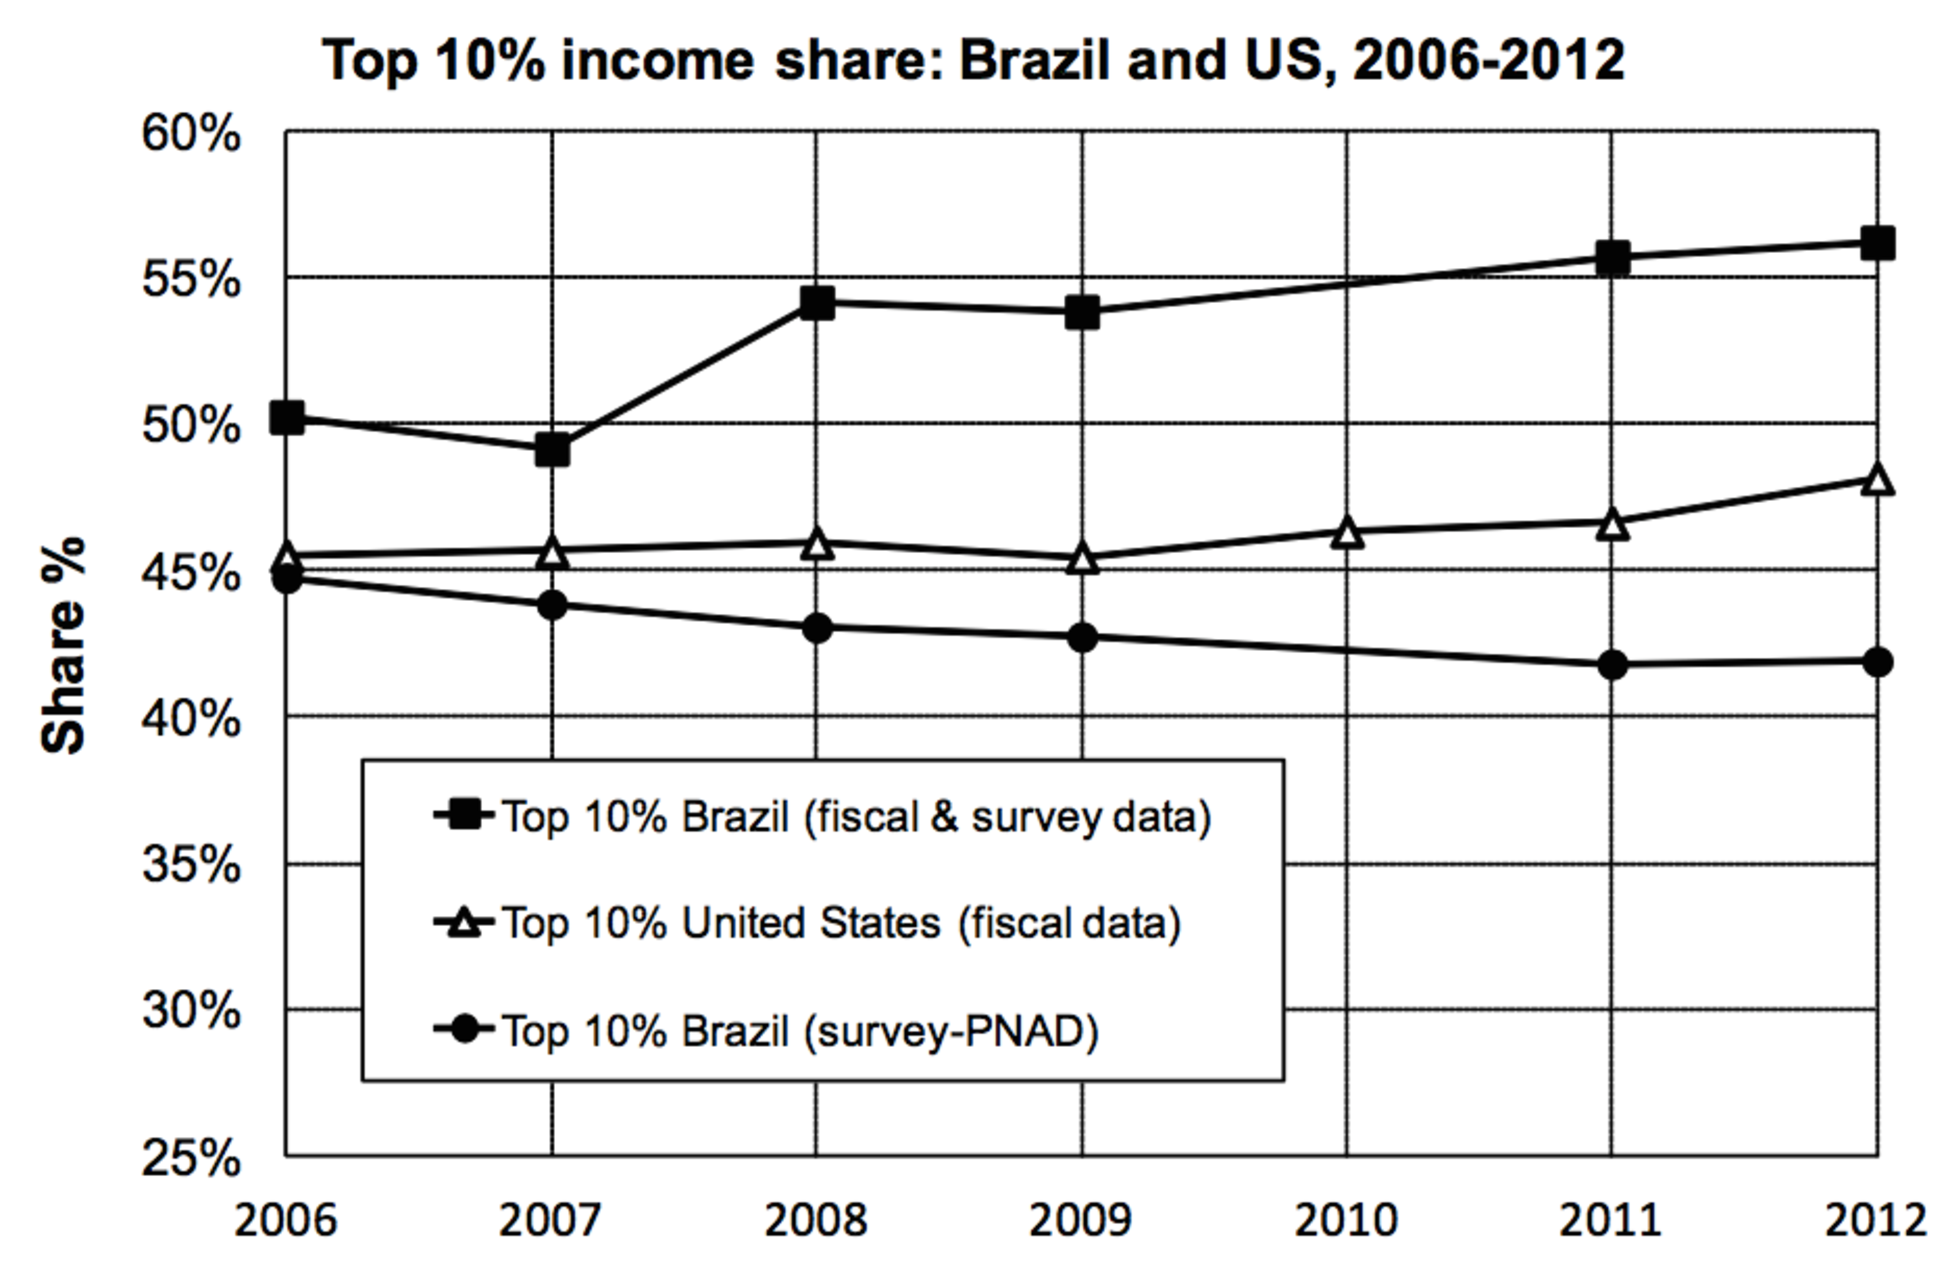
\includegraphics[width=\textwidth]
{pictures/Top10BrazilVsUSA}
\caption{To Do: Get Data to Recreate Figure}
\end{minipage}
\end{figure}
\end{frame}
%%%%%%%%%%%%%%%%%%%% Frame Here %%%%%%%%%%%%%%%%%%%%%%%%%%%%%%%%%%%%%%%%%%%%%%%%


%%%%%%%%%%%%%%%%%%%% Frame Here %%%%%%%%%%%%%%%%%%%%%%%%%%%%%%%%%%%%%%%%%%%%%%%%
\begin{frame}[label=BrazilInequality]
\frametitle{Income Inequality in Brazil: 1976--2013}
\begin{figure}[t]
\begin{minipage}[b]{\textwidth}
\centering
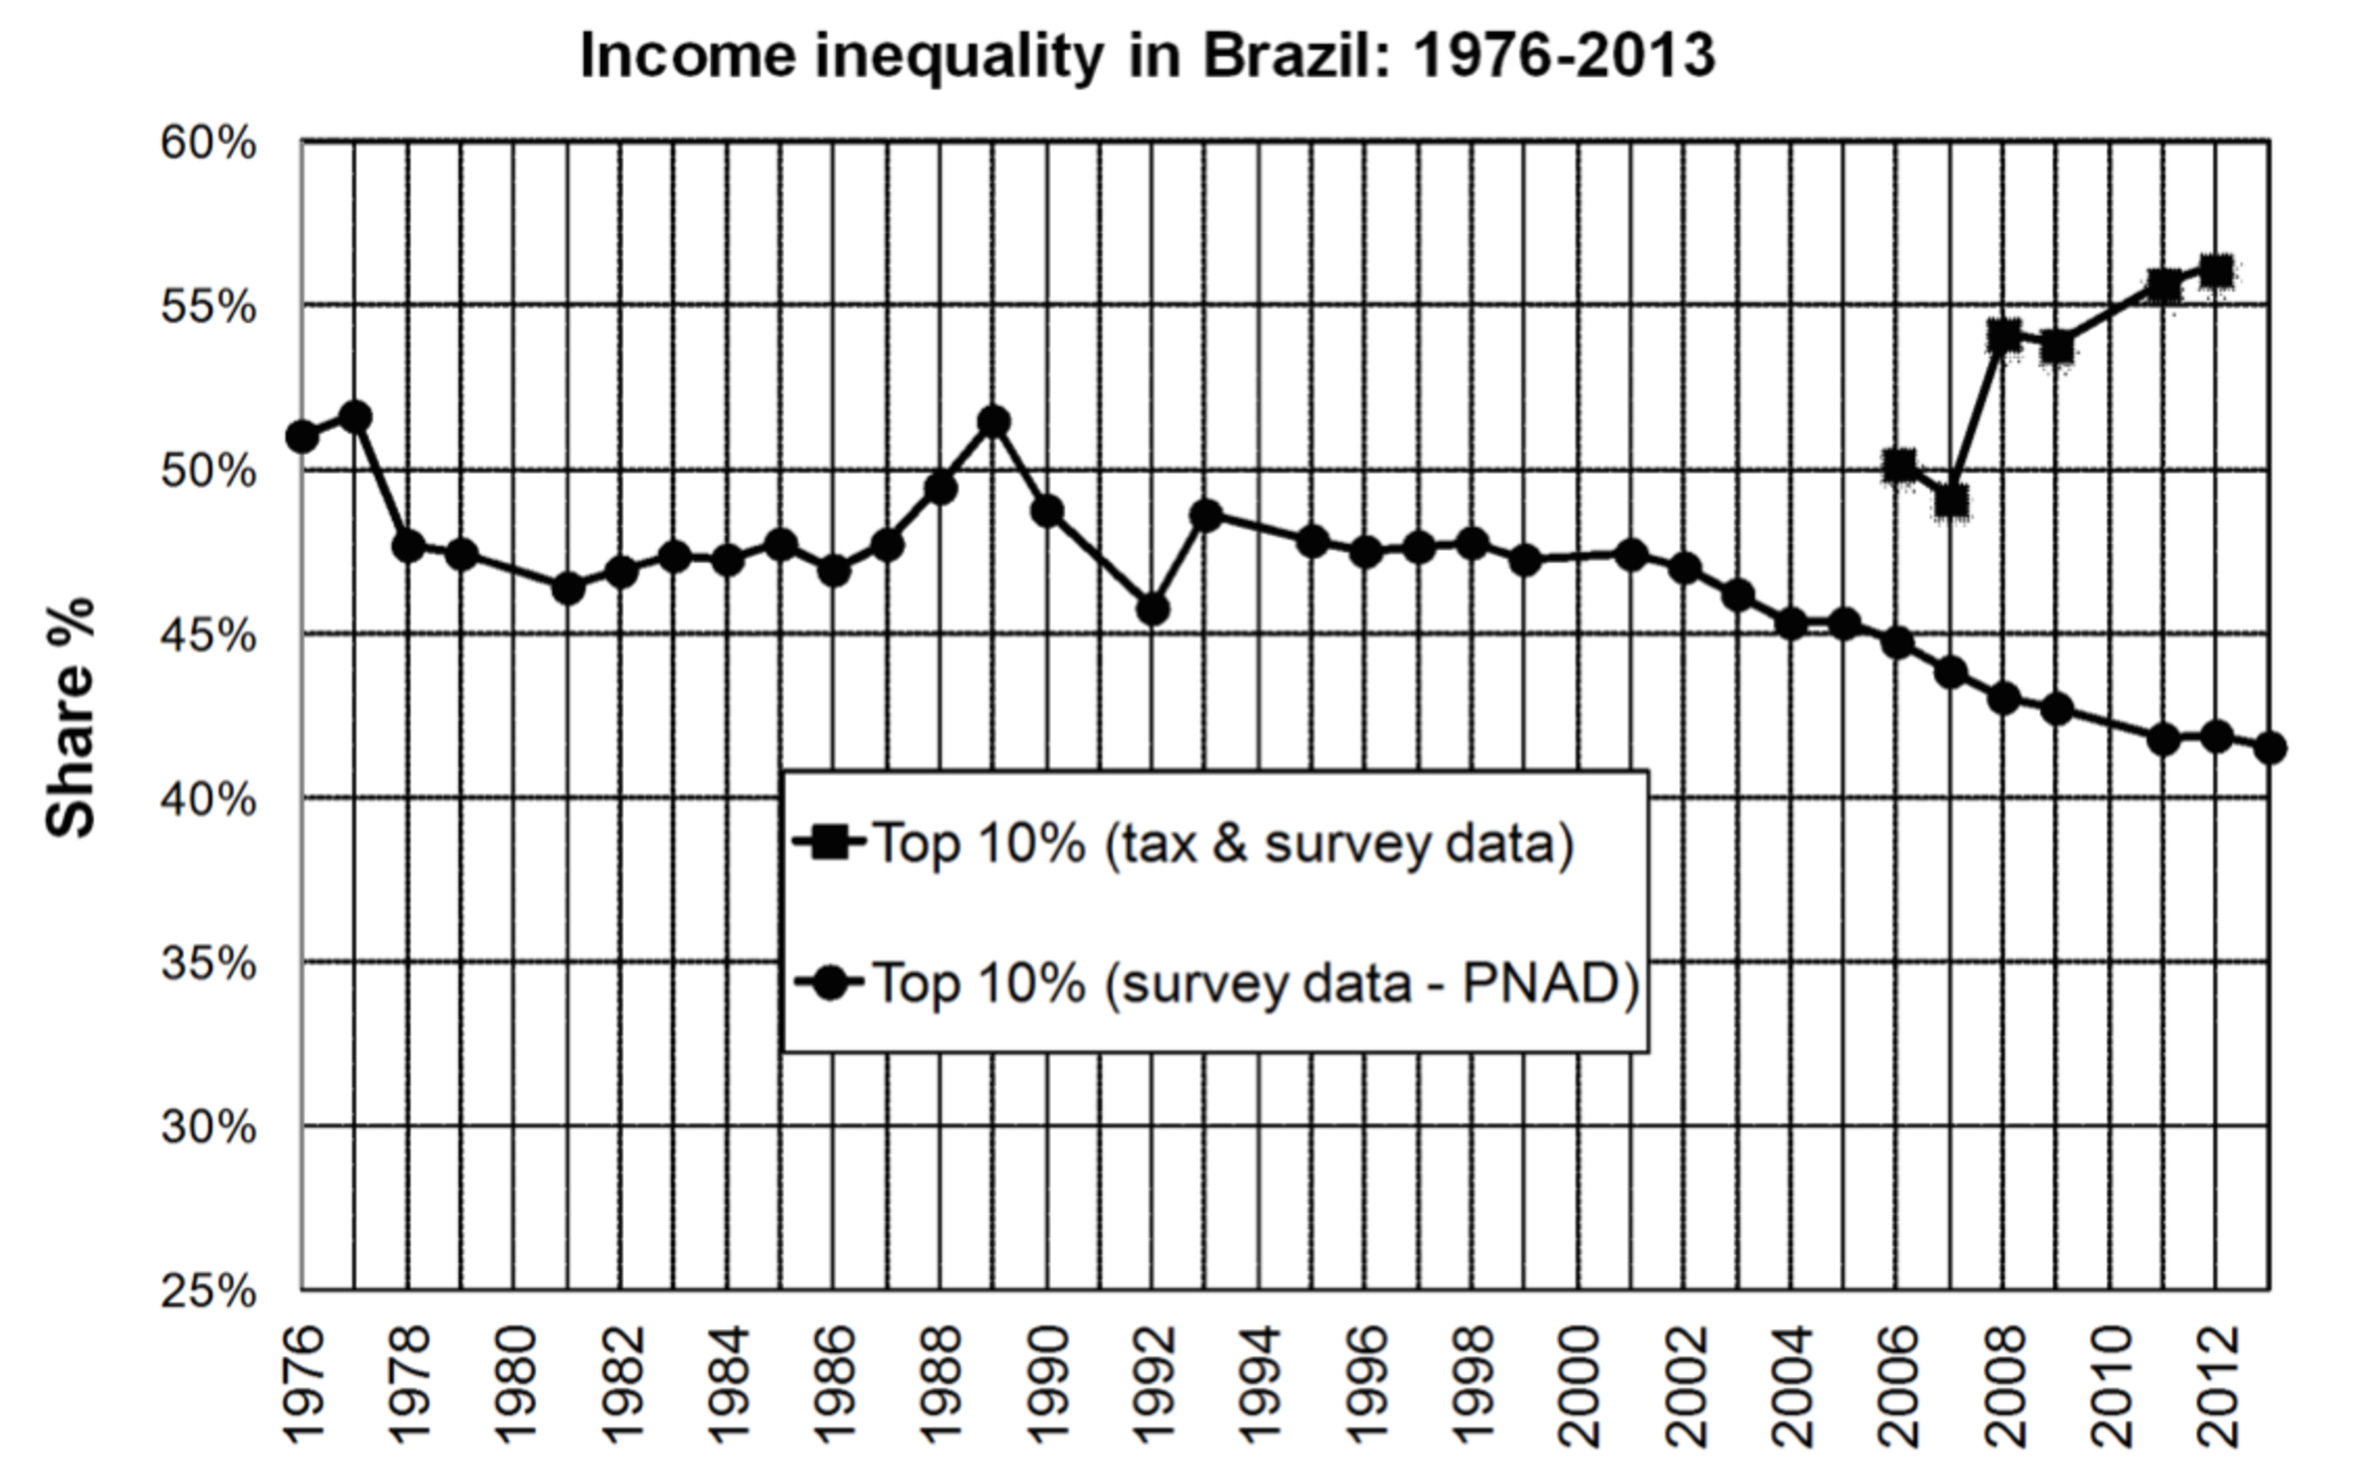
\includegraphics[width=\textwidth]
{pictures/IncomeInequalityBrazil}
\caption{To Do: Get Data to Recreate Figure}
\end{minipage}
\end{figure}
\end{frame}
%%%%%%%%%%%%%%%%%%%% Frame Here %%%%%%%%%%%%%%%%%%%%%%%%%%%%%%%%%%%%%%%%%%%%%%%%


%%%%%%%%%%%%%%%%%%%% Frame Here %%%%%%%%%%%%%%%%%%%%%%%%%%%%%%%%%%%%%%%%%%%%%%%%
%\againframe{ThreePoints}% This seems to be buggy
%%%%%%%%%%%%%%%%%%%% Frame Here %%%%%%%%%%%%%%%%%%%%%%%%%%%%%%%%%%%%%%%%%%%%%%%%


%%%%%%%%%%%%%%%%%%%% Frame Here %%%%%%%%%%%%%%%%%%%%%%%%%%%%%%%%%%%%%%%%%%%%%%%%
\begin{frame}[label=Figure53]
\frametitle{Figure 5.3: Private capital in rich countries, 1970--2010}
\begin{figure}[t]
\begin{minipage}[b]{\textwidth}
\centering
\begin{knitrout}\footnotesize
\definecolor{shadecolor}{rgb}{0.969, 0.969, 0.969}\color{fgcolor}

{\centering 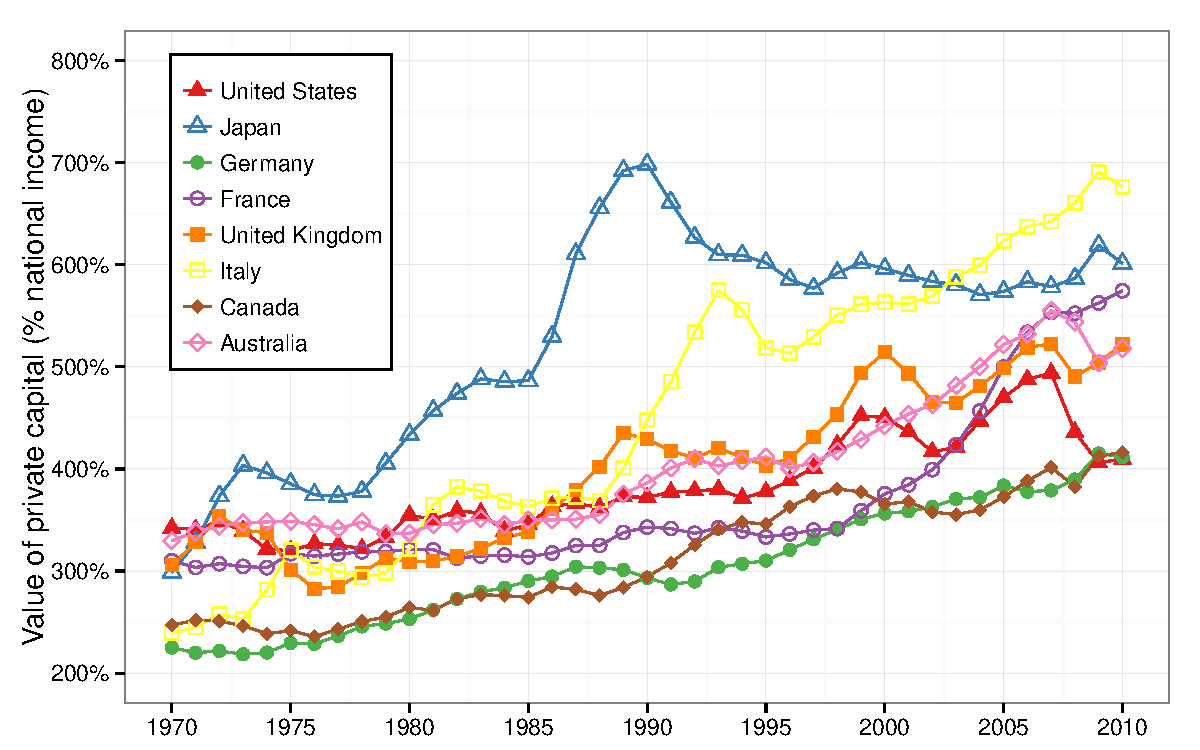
\includegraphics[width=1\linewidth]{figures/color/Figure_5_3} 

}



\end{knitrout}
\caption{Private capital is worth between 2 and 3.5 years of national income in rich countries in 1970, and between 4 and 7 years of national income in 2010.}
\end{minipage}
\end{figure}
\end{frame}
%%%%%%%%%%%%%%%%%%%% Frame Here %%%%%%%%%%%%%%%%%%%%%%%%%%%%%%%%%%%%%%%%%%%%%%%%


%%%%%%%%%%%%%%%%%%%% Frame Here %%%%%%%%%%%%%%%%%%%%%%%%%%%%%%%%%%%%%%%%%%%%%%%%
\begin{frame}[label=Figure54]
\frametitle{Figure 5.4: Private capital in rich countries (ratio), 1970--2010}
\begin{figure}[t]
\begin{minipage}[b]{\textwidth}
\centering
\begin{knitrout}\footnotesize
\definecolor{shadecolor}{rgb}{0.969, 0.969, 0.969}\color{fgcolor}

{\centering 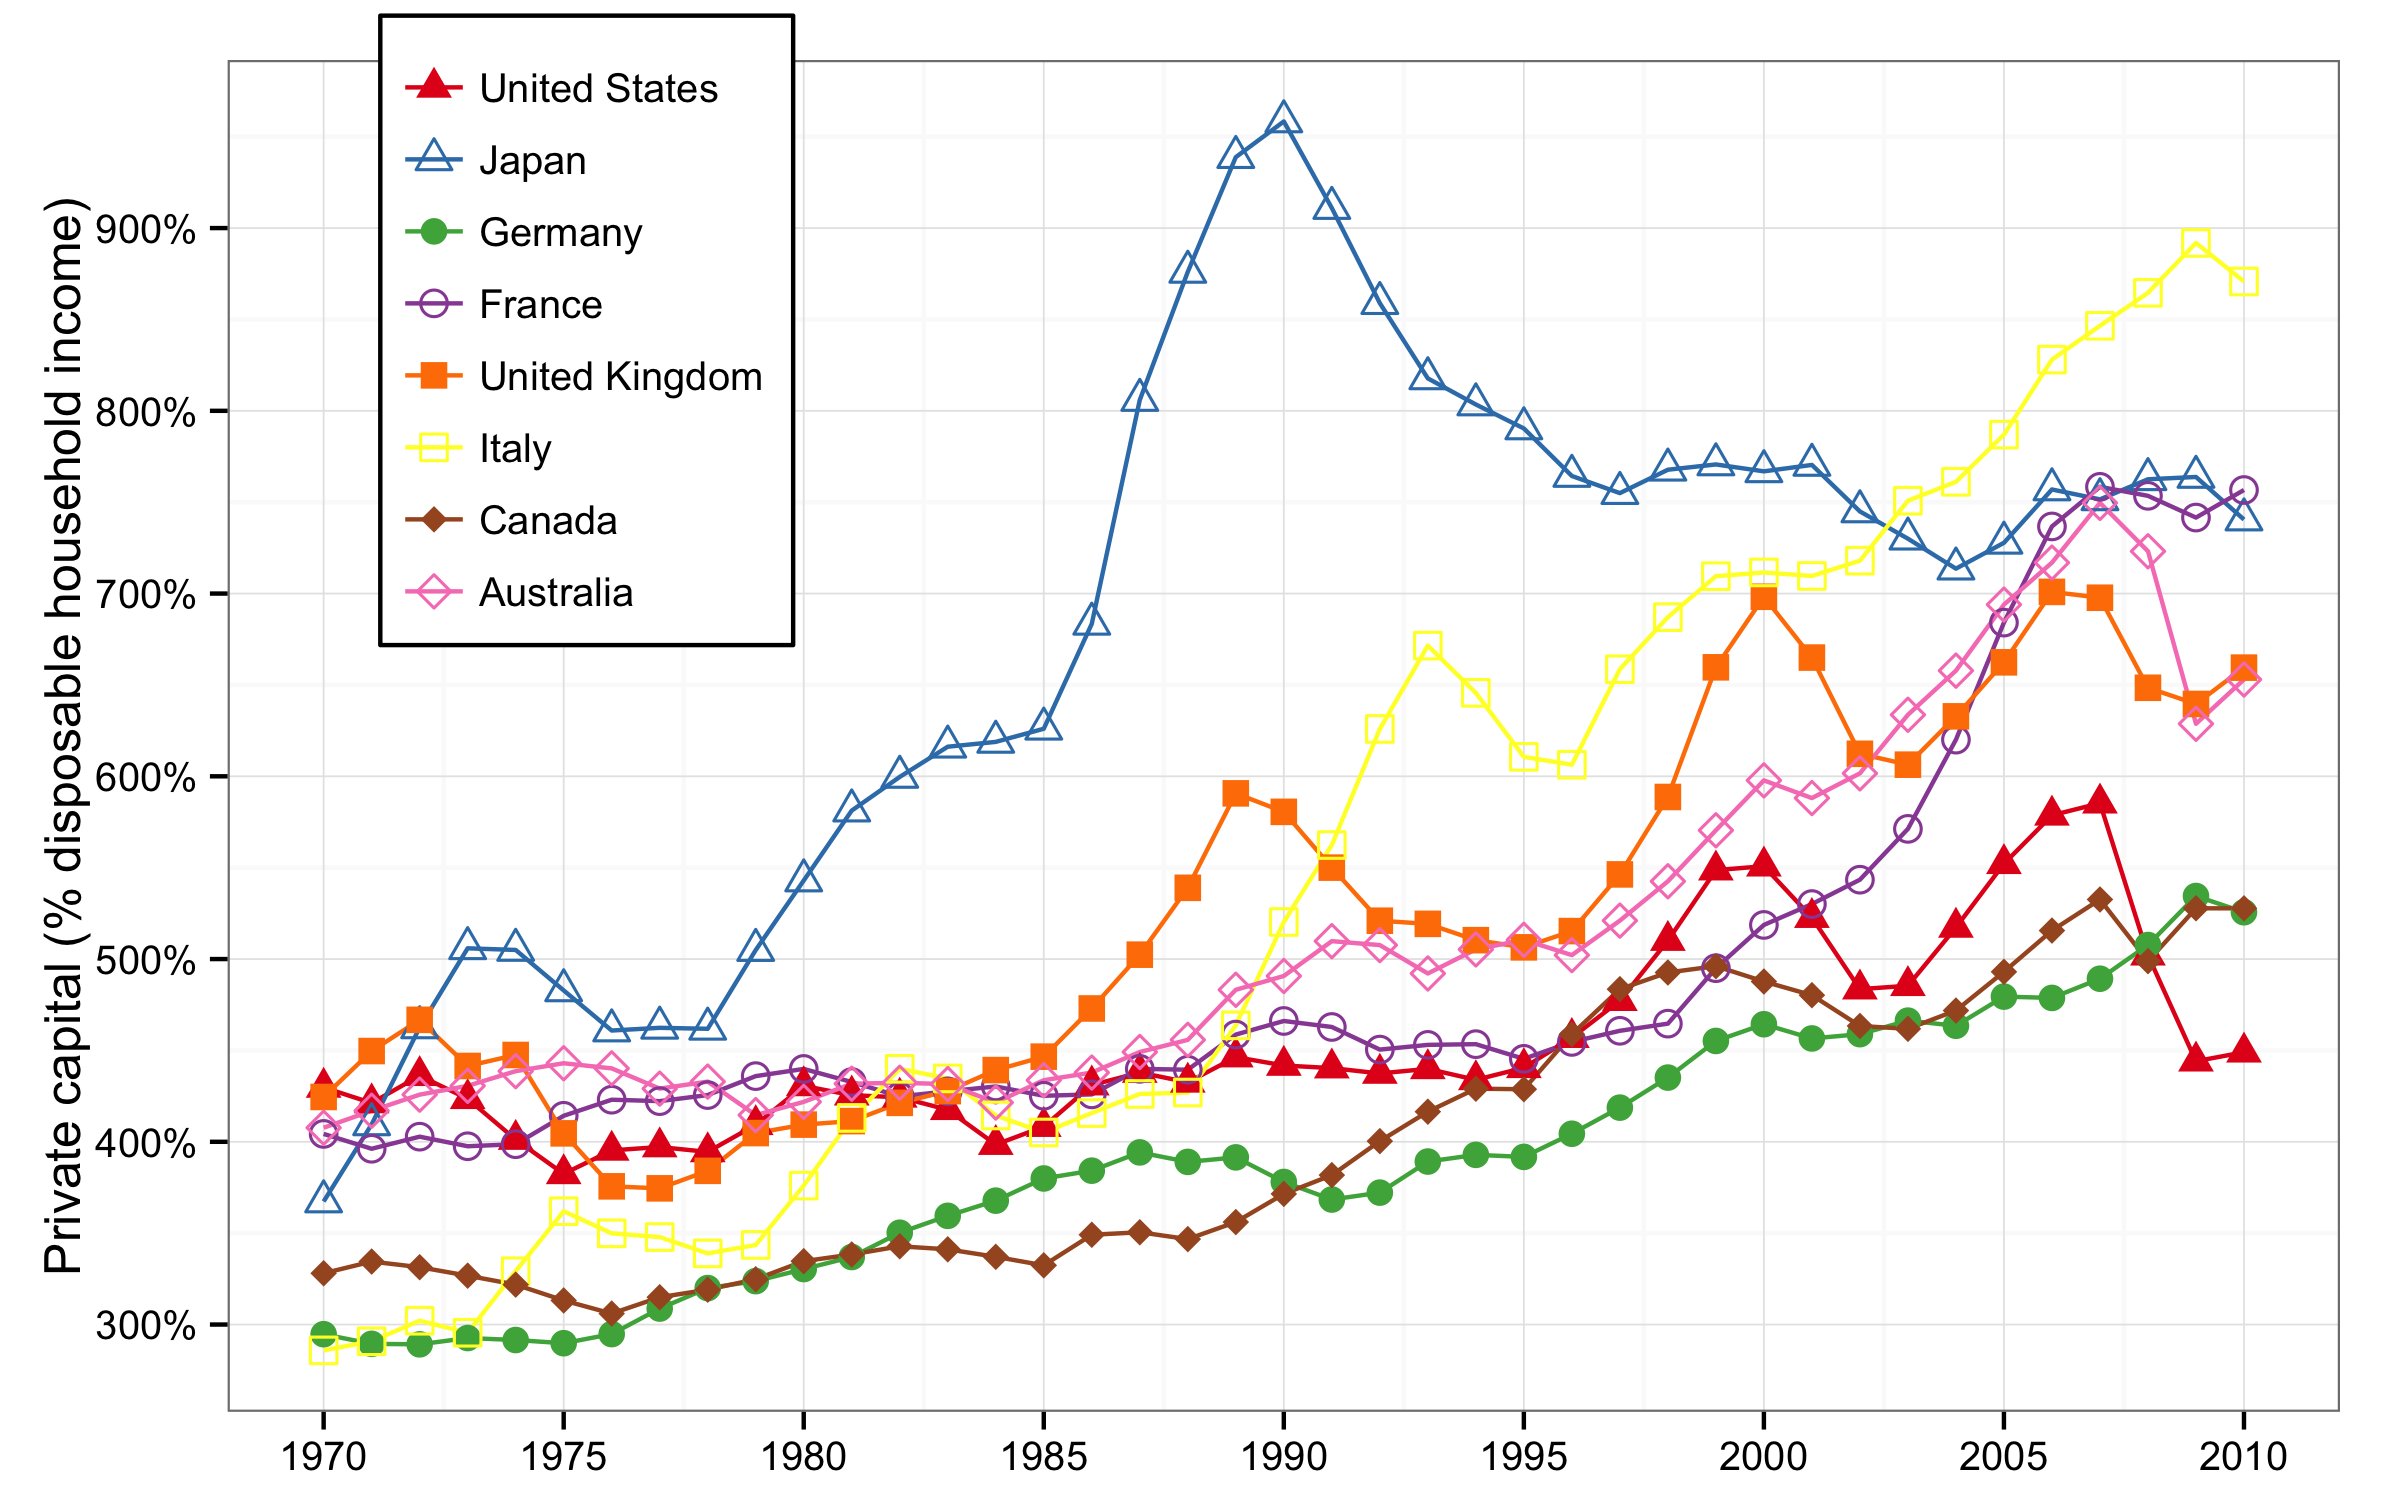
\includegraphics[width=1\linewidth]{figures/color/Figure_5_4} 

}



\end{knitrout}
\caption{Expressed in years of household disposable income (about 70--80\% of national income), the capital/income ratio appears to be larger than when it is expressed in years of national income.}
\end{minipage}
\end{figure}
\end{frame}
%%%%%%%%%%%%%%%%%%%% Frame Here %%%%%%%%%%%%%%%%%%%%%%%%%%%%%%%%%%%%%%%%%%%%%%%%


%%%%%%%%%%%%%%%%%%%% Frame Here %%%%%%%%%%%%%%%%%%%%%%%%%%%%%%%%%%%%%%%%%%%%%%%%
\begin{frame}[label=Figure55a]
\frametitle{Figure 5.3b: Public capital in rich countries, 1970--2010}
\begin{figure}[t]
\begin{minipage}[b]{\textwidth}
\centering
\begin{knitrout}\footnotesize
\definecolor{shadecolor}{rgb}{0.969, 0.969, 0.969}\color{fgcolor}

{\centering 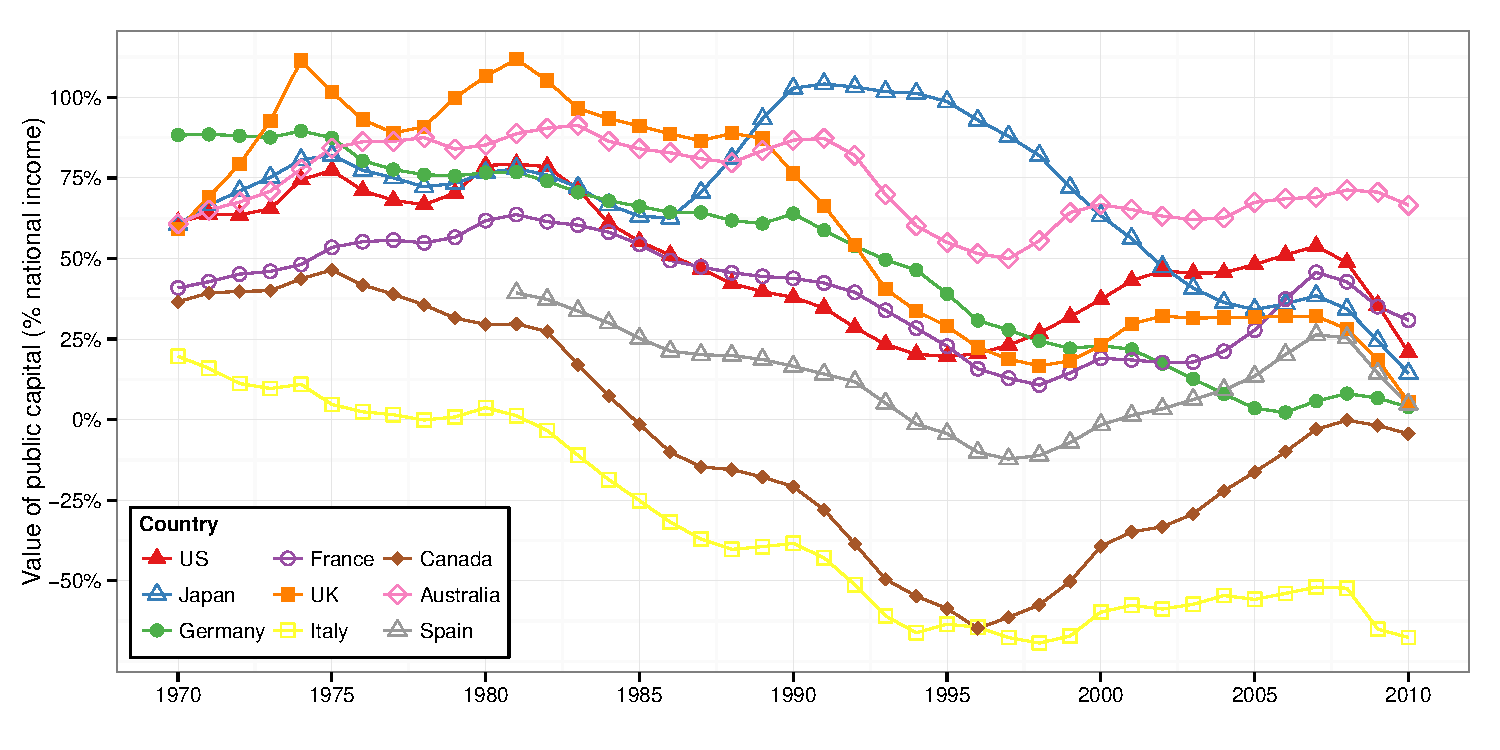
\includegraphics[width=1\linewidth]{figures/color/Figure_5_3b} 

}



\end{knitrout}
\caption{In France, Britain, Germany, and the United States, government deficits exceeded public investment by 2--3\% of national income on average over the period 1970--2010, compared with more than 6\% in Italy.}
\end{minipage}
\end{figure}
\end{frame}
%%%%%%%%%%%%%%%%%%%% Frame Here %%%%%%%%%%%%%%%%%%%%%%%%%%%%%%%%%%%%%%%%%%%%%%%%


%%%%%%%%%%%%%%%%%%%% Frame Here %%%%%%%%%%%%%%%%%%%%%%%%%%%%%%%%%%%%%%%%%%%%%%%%
\begin{frame}[label=Figure55]
\frametitle{Figure 5.5: Private and public capital in rich countries, 1970--2010}
\begin{figure}[t]
\begin{minipage}[b]{\textwidth}
\centering
\begin{knitrout}\footnotesize
\definecolor{shadecolor}{rgb}{0.969, 0.969, 0.969}\color{fgcolor}

{\centering 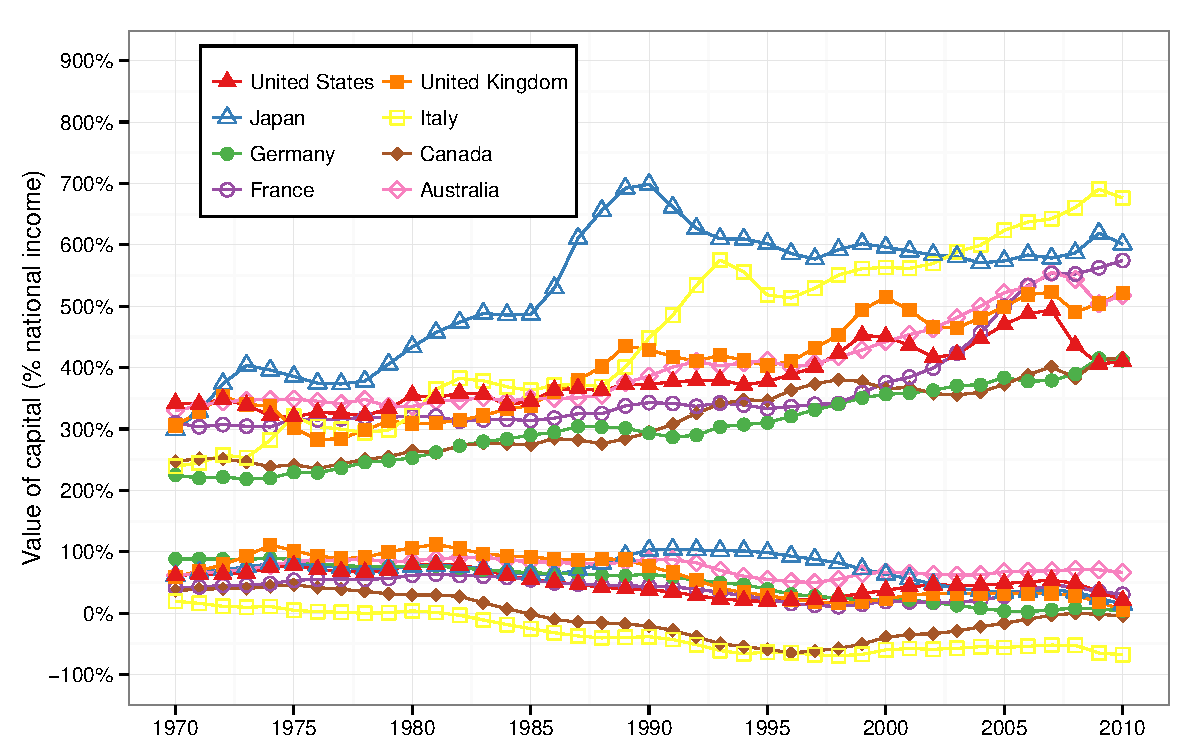
\includegraphics[width=1\linewidth,height=0.75\textheight]{figures/color/Figure_5_5} 

}



\end{knitrout}
\caption{In Italy, private capital rose from 240\% to 680\% in national income between 1970 and 2010, while public capital dropped from 20\% to -70\%.}
\end{minipage}
\end{figure}
\end{frame}
%%%%%%%%%%%%%%%%%%%% Frame Here %%%%%%%%%%%%%%%%%%%%%%%%%%%%%%%%%%%%%%%%%%%%%%%%


%%%%%%%%%%%%%%%%%%%% Frame Here %%%%%%%%%%%%%%%%%%%%%%%%%%%%%%%%%%%%%%%%%%%%%%%%
\begin{frame}[label=Table121]
\frametitle{Table 12.1: The growth rate of top global wealth, 1987--2013}
\begin{table}[t]
%\caption{The growth rate of top global wealth, 1987--2013}
\adjustbox{max height=\dimexpr\textheight-5.5cm\relax,
           max width=\textwidth}{%
\begin{threeparttable}
\centering
\begin{tabular}{@{}lc@{}}
\toprule
    & Average real growth rate per year  \\
    & (after deduction of inflation) (\%) \\
\midrule
    The top 1/(100 million) highest wealth holders \tnote{a}   & 6.8  \\
    The top 1/(20 million)  highest wealth holders \tnote{b}   & 6.4  \\
    Average world wealth per adult                             & 2.1  \\
    Average world income per adult                             & 1.4  \\
    World adult population                                     & 1.9  \\
    World GDP                                                  & 3.3  \\
\midrule
\end{tabular}
\begin{tablenotes}
    \item Between 1987 and 2013, the highest global wealth fractiles have grown at 6--7\% per year versus 2.1\% for average world wealth, and 1.4\% for average world income. All growth rates are net of inflation (2.3\% per year between 1987 and 2013).
    \item[a] About 30 adults out of 3 billion in the 1980s, and 45 adults out of 4.5 billion in 2010.
    \item[b] About 150 adults out of 3 billion in the 1980s, and 225 adults out of 4.5 billion in the 2010s.
\end{tablenotes}
\end{threeparttable}}
\end{table}
\end{frame}
%%%%%%%%%%%%%%%%%%%% Frame Here %%%%%%%%%%%%%%%%%%%%%%%%%%%%%%%%%%%%%%%%%%%%%%%%


%%%%%%%%%%%%%%%%%%%% Frame Here %%%%%%%%%%%%%%%%%%%%%%%%%%%%%%%%%%%%%%%%%%%%%%%%
\begin{frame}[label=Table122]
\frametitle{Table 12.2: The return on the capital endowments of U.S. universities, 1980--2010}
\begin{table}[t]
%\caption{The return on the capital endowments of U.S. universities, 1980--2010}
\adjustbox{max height=\dimexpr\textheight-5.5cm\relax,
           max width=\textwidth}{%
\begin{threeparttable}
\centering
\begin{tabular}{@{}lc@{}}
\toprule
    & Average real annual rate of return                           \\
    & (after deduction of inflation and all                        \\
    & administrative costs and financial fees) (\%)                \\
\midrule
    All universities (850)                                & 8.2    \\
    Harvard, Yale, and Princeton                          & 10.2   \\
    Endowments higher than \$1 billion (60)               & 8.8    \\
    Endowments between \$500 million and 1 billion (66)   & 7.8    \\
    Endowments between \$100 and \$500 million (226)      & 7.1    \\
    Endowments less than \$100 million (498)              & 6.2    \\
\midrule
\end{tabular}
\begin{tablenotes}
    \item Between 1980 and 2010, U.S. universities earned an average real rate of return of 8.2\% on their capital endowments, and more for the greater endowments. All returns are reported net of inflation (2.4\% per year between 1980 and 2010) and net of administrative costs and financial fees.
\end{tablenotes}
\end{threeparttable}}
\end{table}
\end{frame}
%%%%%%%%%%%%%%%%%%%% Frame Here %%%%%%%%%%%%%%%%%%%%%%%%%%%%%%%%%%%%%%%%%%%%%%%%


%%%%%%%%%%%%%%%%%%%% Frame Here %%%%%%%%%%%%%%%%%%%%%%%%%%%%%%%%%%%%%%%%%%%%%%%%
\begin{frame}[label=Figure98]
\frametitle{Figure 9.8: Income inequality: Europe vs. United States, 1900--2010}
\begin{figure}[t]
\begin{minipage}[b]{\textwidth}
\centering
\begin{knitrout}\footnotesize
\definecolor{shadecolor}{rgb}{0.969, 0.969, 0.969}\color{fgcolor}

{\centering 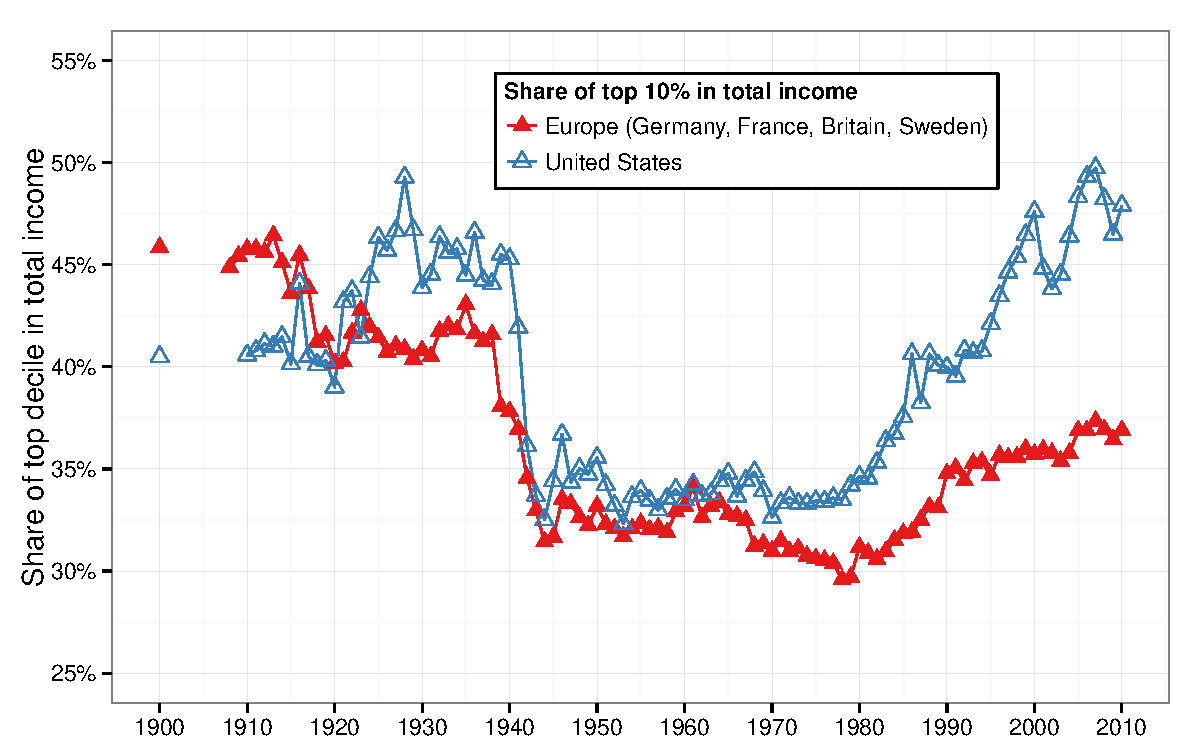
\includegraphics[width=1\linewidth]{figures/color/Figure_9_8} 

}



\end{knitrout}
\caption{The top decile income share was higher in Europe than in the U.S. in 1900-2010. It is much higher in the U.S. in 2000-2010.}
\end{minipage}
\end{figure}
\end{frame}
%%%%%%%%%%%%%%%%%%%% Frame Here %%%%%%%%%%%%%%%%%%%%%%%%%%%%%%%%%%%%%%%%%%%%%%%%


%%%%%%%%%%%%%%%%%%%% Frame Here %%%%%%%%%%%%%%%%%%%%%%%%%%%%%%%%%%%%%%%%%%%%%%%%
\begin{frame}[label=Figure141]
\frametitle{Figure 14.1: Top income tax rates, 1900--2013}
\begin{figure}[t]
\begin{minipage}[b]{\textwidth}
\centering
\begin{knitrout}\footnotesize
\definecolor{shadecolor}{rgb}{0.969, 0.969, 0.969}\color{fgcolor}

{\centering 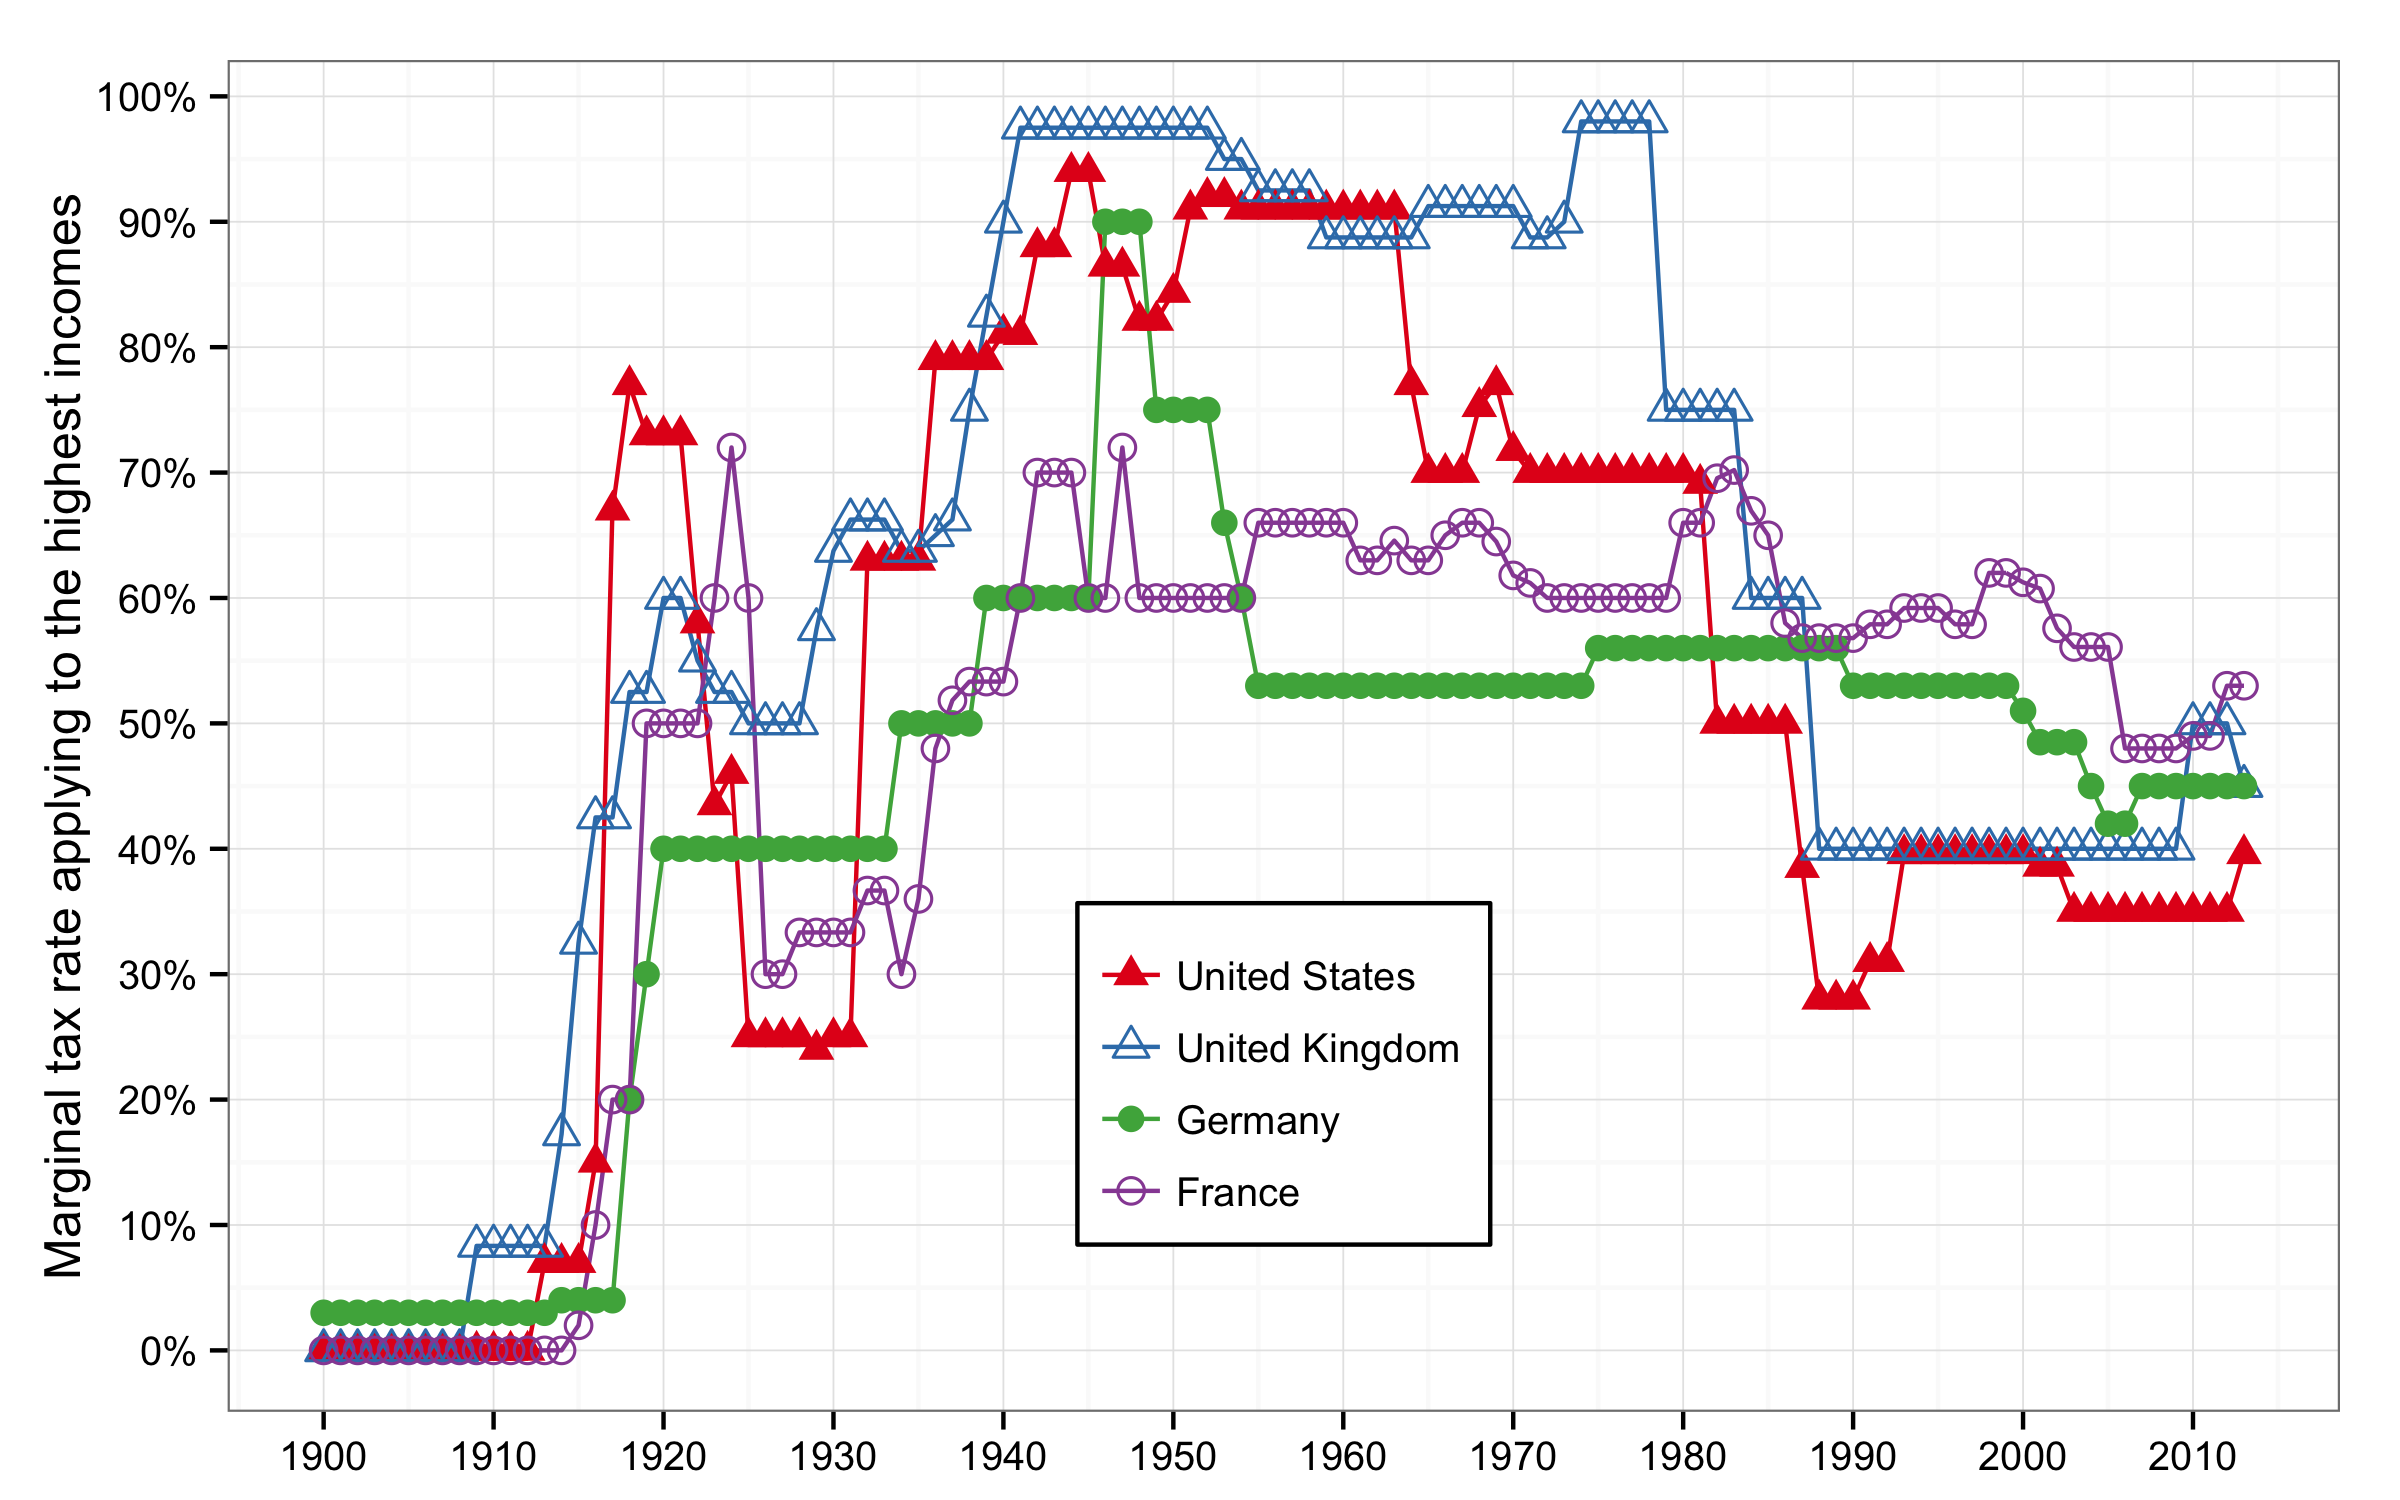
\includegraphics[width=1\linewidth]{figures/color/Figure_14_1} 

}



\end{knitrout}
\caption{The top marginal tax rate of the income tax (applying to the highest incomes) in the U.S. dropped from 70\% in 1980 to 28\% in 1988.}
\end{minipage}
\end{figure}
\end{frame}
%%%%%%%%%%%%%%%%%%%% Frame Here %%%%%%%%%%%%%%%%%%%%%%%%%%%%%%%%%%%%%%%%%%%%%%%%


%%%%%%%%%%%%%%%%%%%% Frame Here %%%%%%%%%%%%%%%%%%%%%%%%%%%%%%%%%%%%%%%%%%%%%%%%
\begin{frame}[label=Figure142]
\frametitle{Figure 14.2: Top inheritance tax rates, 1900--2013}
\begin{figure}[t]
\begin{minipage}[b]{\textwidth}
\centering
\begin{knitrout}\footnotesize
\definecolor{shadecolor}{rgb}{0.969, 0.969, 0.969}\color{fgcolor}

{\centering 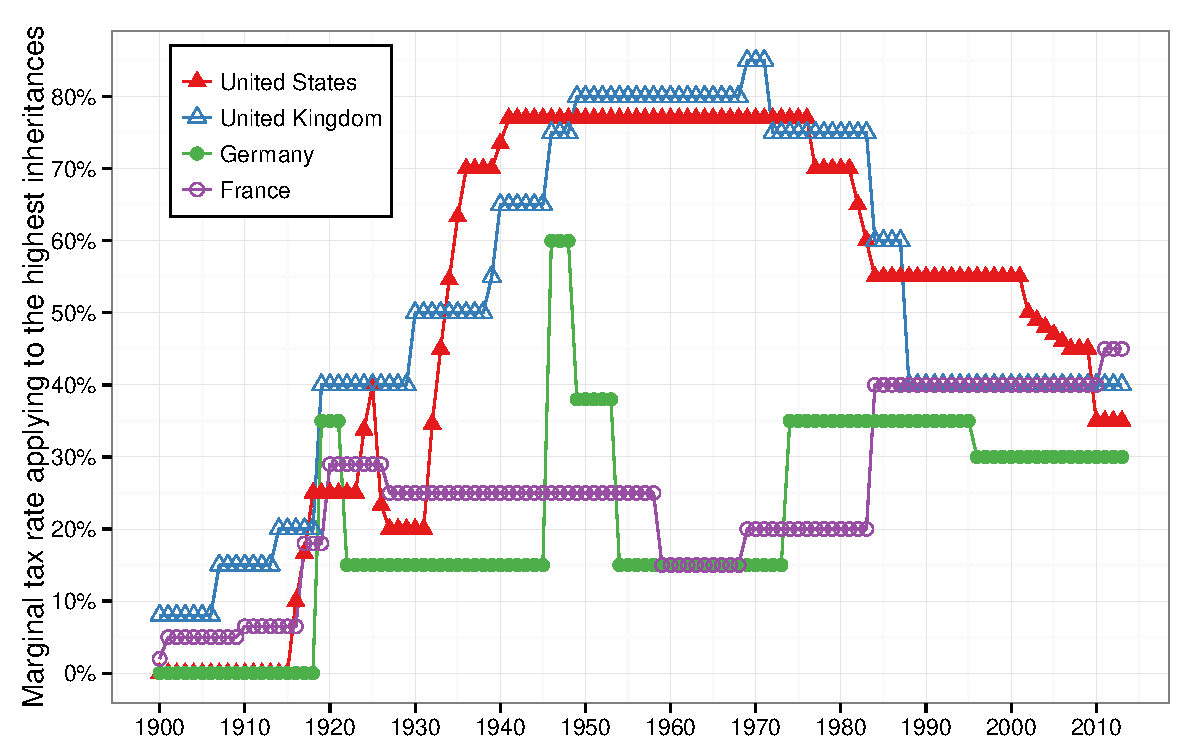
\includegraphics[width=1\linewidth]{figures/color/Figure_14_2} 

}



\end{knitrout}
\caption{The top marginal tax rate of the inheritance tax (applying to the highest inheritances) in the U.S. dropped from 70\% in 1980 to 35\% in 2013.}
\end{minipage}
\end{figure}
\end{frame}
%%%%%%%%%%%%%%%%%%%% Frame Here %%%%%%%%%%%%%%%%%%%%%%%%%%%%%%%%%%%%%%%%%%%%%%%%


%%%%%%%%%%%%%%%%%%%% Frame Here %%%%%%%%%%%%%%%%%%%%%%%%%%%%%%%%%%%%%%%%%%%%%%%%
\begin{frame}[label=Conclusions1]
\frametitle{Conclusions}
\begin{itemize}
\item
The history of income and wealth inequality is always political, chaotic and unpredictable; it involves national identities and sharp reversals; nobody can predict the reversals of the future
\item
Marx: with $g=0$, $\beta\rightarrow\infty$, $r\rightarrow 0$ : revolution, war
\item
My conclusions are less apocalyptic: with $g>0$, at least we have a steady state $\beta=s/g$
\item
But with $g>0$ \& small, this steady-state can be rather gloomy: it can involve a very large capital-income ratio $\beta$ and capital share $\alpha$, as well as extreme wealth concentration due to high $r-g$
\item
This has nothing to do with a market imperfection: the more perfect the capital market, the higher $r-g$
\item
The ideal solution: progressive wealth tax at the global scale, based upon automatic exchange of bank information
\item
Other solutions involve authoritarian political \& capital controls (China, Russia..), or perpetual population growth (US), or inflation, or some mixture of all
\end{itemize}
\end{frame}
%%%%%%%%%%%%%%%%%%%% Frame Here %%%%%%%%%%%%%%%%%%%%%%%%%%%%%%%%%%%%%%%%%%%%%%%%


\end{document}
